\documentclass{trkut}% Reaalkooli vormistus. Muidu "report" või "article".
\usepackage[style=trkut]{biblatex}% Kasutatud kirjanduse genereerimine
\addbibresource{viited_eesnimi_perekonnanimi.bib}% Viidete info fail
\defbibheading{bibliography}{\addchap{#1}}% Lisame kasutatud materjalid sisukorda

\pealkiri{Atmosfääri mudeldamine ja katseandmete põhjal täpseima mudeli leidmine} % Kahel real
\autor{Jarl Patrick Paide}
\klass{11.a}
\juhendaja{õp. Mart Kuurme \\ õp. Kaarel Kivisalu}% Toetab praegu ainult ühte juhendajat, manual fix: muuda cls failis juhendaja -> juhendajad

\begin{document}
\maketitle% Tiitelleht
\tableofcontents% Sisukord

\addchap{Sissejuhatus}
\nummerdame% See käsk peab olema kohe peale sissejuhatust
%See teema on aktuaalne, kuna see on väga huvitav ja ma tahan seda uurida...


\chapter{Teooria}
Teooria osas proovitakse leida erinevaid täpseid viise kuidas kirjeldada rõhu ja temperatuuri sõltuvust kõrgusest. 

\begin{figure}[h]
	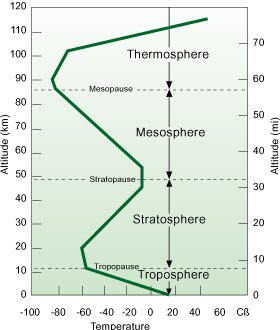
\includegraphics[width=1\textwidth]{profile.png}
	\caption{Kõrguse sõltuvus ajast}
	%\allikas{Minu programm}
	\label{profile}% Selle järgi viidatakse, see rida peab olema pärast \caption
\end{figure}

Joonisel \ref{profile} on näha kuidas temperatuur muutub kõrguse kasvades. Troposfääris temperatuur langeb ja stratosfääris temberratuur tõuseb. Kõrguse kasvades rõhk väheneb, sest kõrguse kasvades väheneb üleval pool oleva õhu mass mis surub õhku kokku poole tekidades rõhku. Kuna rõhk väheneb siis temperatuur langeb. See seletab temperatuuri langust troposfääris. Peale troposfääri tuleb osoonikiht mis asub stratosfääris. Osoon neelab päikeselt tulevat kiirgust muutes selle soojuseks. Mida kõrgemal seda vähem kiirgust on neelatud päikese poolt, seda soojem. Sellega piirdub meid huvitatav piirkond.

Selles peatükkis on avaldatud temperatuuri ja rõhu sõltuvused kõrgusest erinevate meetoditega otsides kõige täpsemat kirjeldust.

Termodünaamika esimene seadus on
\begin{equation}\label{eq1}
dU = dQ - dA
\end{equation}

\section{Ideaalne gaas}
Teeme lihtsustuse, et gaasid atmosfääris on ideaalsed. Siis saame kasutada ideaalse gaasi olekuvõrrandid
\begin{equation}\label{eq8}
PV=\nu RT
\end{equation}

\subsection{Erisoojustest}
Gaasi siseenergia $U$ avaldub vabadusastmete $i$ kaudu järgneva seaose abil.
\begin{equation}\label{eq5}
U = \frac{i}{2} \nu R T
\end{equation}
Konstanstse ruumala puhul tööd ei tehta, seega kogu soojus läheb siseenergia suurendamiseks. Saame soojusmahutavuse võttes siseenergia muudust tuletist temeratuuri järgi.
\begin{equation}\label{eq6}
C_V = \frac{dU}{dT}=\frac{i}{2}\nu R
\end{equation}
Molaarset soojusmahutavust saab avaldada valemiga $c_V = \frac{C_V}{\nu}$ saades molaarseks soojusmahutavuseks
\begin{equation}\label{eq7}
c_V = \frac{i}{2}R
\end{equation}

Kui aga vaadata isobaarilist protsessi siis vaadates olekuvõrrendid tuleneb $pdV=\nu RdT$, ning gaas teeb tööd $dA = pdV = \nu RdT$. Avaldades need valemisse \ref{eq1} saame
\begin{equation}
dQ = dU + dA = \frac{i+2}{2} \nu R dT
\end{equation}
Millest järeldub
\begin{equation}
c_p=\frac{i+2}{2}R
\end{equation}
Sammuti saab näidata $c_V$ ja $c_p$ vahelist seost
\begin{equation}\label{eq9}
c_p = c_V + R
\end{equation}
          
\subsection{Adiabaatiline protsess}
Adiabaatiline protsess on termodünaamiline protsess mille käigus ei toimus soojusvahetust väliskeskonnaga. Kuna atmosfääris on õhud pidevas üles-alla liikumises siis soojusvahetust ei toimu.

Harilikult on õhumassid atmosfääris tugevas liikumises, nii et nad liiguvad pidevalt üles-alla. Et kõrgemal on rõhk väiksem, kui all, siis jahtub gaas üles liikudes heas lähenduses adiabaatilise paisumise tõttu (õhumasside suurte mõõtmete tõttu on soojusjuhtivus hästi aeglane).

% Jaan kalda
% Adiabaatiliseks nimetatakse sellist protsessi, mis on nii aeglane, et tema kulgemise karakteerne aeg on mõnevõrra väiksem (praktikas piisab paarikordset erinevusest), kui süsteemi omavõnkesagedus.


Kuna adiabaatilises protsessis soojusvahetust ei toimu siis valemis \ref{eq1} $dQ=0$. Gaasi poolt tehtud töö on $d A=pdV$ ja gaasi siseenergia muut on $dU=\nu c_VdT$. Sellest järeldub:
\begin{equation}\label{eq2}
\nu c_VdT = -pdV
\end{equation}
Ideaalse gaasi olekuvõrrandist \ref{eq8} saame tuletist võttes ja avaldades järgneva
\begin{equation}\label{eq3}
dT = \frac{pdV+Vdp}{\nu R}
\end{equation}

Asendades \ref{eq3} valemi valemisse \ref{eq2} saame uue seose.
\begin{equation}\label{eq4}
pdV(c_V+R)+c_VVdp=0
\end{equation}
Asendame siia sisse valemi \ref{eq9} ja adiabaadinäitaja
\begin{equation}
\gamma \equiv \frac{c_p}{c_V}
\end{equation}
Nüüd eelmisi seoseid kasutades ja ümber paigudades saame võrrandi
\begin{equation}
\gamma \frac{dV}{V} + \frac{dp}{p} = 0
\end{equation}
Seda integreerides saame
\begin{equation}
 \int \gamma \frac{dV}{V} + \frac{dp}{p} = \gamma \ln(V) + \ln(p) = Const.
\end{equation}
Sellest saame järeldada
\begin{equation}
pV^\gamma = Const.
\end{equation}
Sammuti kasutades ideaalse gaasi olekuvõrrandid saame tuletada veel 2 seost
\begin{equation}\label{eq13}
p^{1-\gamma}T^\gamma = Const.
\end{equation}
\begin{equation}
V^{\gamma-1}T = Const.
\end{equation}

\subsection{Rõhu muutus atmosfääris}
Vaatame õhukest õhuriba laiusega $dz$. Rõhu muutust selle kõrguse vahel saab kirjeldada valemiga
\begin{equation}\label{eq10}
dp=-\rho gdz
\end{equation}
Õhu tihedust on võimalik kirjeldada järgnevalt kasutades ideaalse gaasi olekuvõrrandit
\begin{equation}\label{eq11}
\rho = \frac{\nu \mu}{V} = \frac{p \mu}{RT}
\end{equation}
Pannes valemid \ref{eq10} ja \ref{eq11} kokku saame
\begin{equation}\label{eq12}
\frac{dp}{p} = -\frac{\mu g}{RT}dz
\end{equation}
Valemist \ref{eq13} saame
\begin{equation}
d\ln(p^{1-\gamma}T^\gamma) = 0
\end{equation}
Millest saame
\begin{equation}
\frac{dp}{p} = \frac{\gamma}{\gamma-1}\frac{dT}{T}
\end{equation}
Pannes see nüüd kokku valemiga \ref{eq12} saame valemi
\begin{equation}
\frac{dT}{dz}=-\frac{\gamma-1}{\gamma} \frac{\mu g}{R}
\end{equation}
Seda integreerides saame
\begin{equation}
T=T_0 \bigg( 1-\frac{\gamma-1}{\gamma} \frac{z}{z_0} \bigg)
\end{equation}
Kus $T_0$ on temperatuur maapinnal ja $z_0 = \frac{RT_0}{\mu g} $. Kasutades nuud seost \ref{eq13} saame seose
\begin{equation}
p = p_0 \bigg( 1-\frac{\gamma-1}{\gamma} \frac{z}{z_0} \bigg)^\frac{\gamma}{\gamma-1}
\end{equation}

\section{Wan der Waals}
Wan der Waalsi esitas ideaalse gaasi olekuvõrrandist täpsema mudeli gaasi olekuvõrrandi jaoks.
\begin{equation}\label{eq15}
\nu RT = \bigg( p+\frac{\nu^2 a}{V^2} \bigg) \bigg( V - \nu b \bigg)
\end{equation}
Kus $ a = ?? $ ja $ b = ??$. Siseenergia on antud
\begin{equation}\label{eq14}
U = \nu c_VT-\frac{\nu^2 a}{V}
\end{equation}


\subsection{Adiabaatiline protsess}
Siseenergia muutu saab avaldada valemist \ref{eq14}
\begin{equation}
dU = \nu c_VdT + \frac{\nu^2 a}{V^2}dV
\end{equation}
Adiabaatilise protsessi deffinitsiooni kohaselt ei anta gaasile siseenergiat juurde, ehk $dQ = 0$. Seega saame kirja panna
\begin{equation}
0 = dU + pdV = \nu c_V dT + \bigg( \frac{\nu^2 a}{V^2} + p \bigg) dV
\end{equation}
Asendades siia sisse valemi \ref{eq15} saame
\begin{equation}
0 = c_V dT + \frac{RT}{V - \nu b}dV
\end{equation}
\begin{equation}
\int - \frac{c_V}{T} dT = \int \frac{R}{V - \nu b}dV
\end{equation}
\begin{equation}
c_V \ln(T) + R \ln(V - \nu b) = Const.
\end{equation}
\begin{equation}
(V - \nu b)^R T^{c_V} = Const.
\end{equation}
\begin{equation}
(V - \nu b)^{R + c_V} \bigg( p + \frac{\nu^2 a}{V^2} \bigg)^{c_V} = Const.
\end{equation}
\begin{equation}
 \bigg( p + \frac{\nu^2 a}{V^2} \bigg) (V - \nu b)^\gamma = Const.
\end{equation}


\chapter{Katsed ja andmete analüüs}
\section{Metoodika}
\subsection{Andmete kogumine}
Andmeid kogutakse heeliumiga täidetud õhupalliga kaasa saadetud sondiga, mis mõõdab erinevaid andmeid. Põhilisteks andmeteks on kõrgus, asukoht, aeg, välistemperatuur ja rõhk. Sondi pardal on Raspberry Pi arvuti. Õhupall kerkib atmosfääri kõrgemadesse kihtidesse, sest üleslükkejõud ületab kerge gaasi ja sondi massi. Kõrgemale tõustes rõhk väheneb. Et õhupalli siserõhk oleks tasakaalus välisrõhuga, suureneb õhupalli ruumala, kuni õhupall lõhkeb ülepingest. Peale seda kukkub sond alla ja leitakse GPS'ga üles.
\subsection{Andmete analüüs}
Andmete analüüsimisks kasutan enda poolt kirjutatud c++/Python programmi. Programmiga saab joonistada graafikuid andmete põhjal ja kontrollida erinevaid seoseid.

\section{Varem tehtud katsed}
Selles uurimistöös tehtud katsed on tehtud Eesti kosmosekoolide võrgustiku siseselt. See võrgustik on varem teinud juba kaks heeliumõhupalli lendu, ning selle uurimistööga seoses tehakse ka heeliumõhupalliga lend. Uue katse planeerimiseks on vajalik eelmiste katsete analüüs ja leida vigu, mida uues katses parandada.
\newline Esimene lend mis tehti 29. märtsil kestis umbes kaks tundi, kus kõrgeim punkt milleni jõuti oli 26474 m. Selleks läks aega poolteist tundi ja sellel kõrgusel lõhkes õhupall väikese välisrõhu pärast suureks paisumise tõttu. Kokku tehti 220 mõõtmist. Mõõtmise alla kuulusid kellaaeg, laiuskraad, pikkuskraad, kõrgus, kapsli sisetemperatuur, välistemperatuur ja rõhk.
\newline Teine lend tehti 11. mail ning seekord kestis lend peaaegu neli tundi, jõudes kolme ja poole tunniga kõrgusele 32608 m. Katse tegijad muutsid õhupallis heeliumi kogust, mille tõttu oli tõusmise kiirus väiksem, aga õhupall plahvatas hiljem ja jõuti kõrgemale. Seekord tehti 4300 mõõtmist ja mõõdeti samu parameetreid.
\newline Ma kasutan teise lennu andmeid, et planeerida enda lendu, sest teisel lennul on tihedamad andmepunktid.

\subsection{Kõrguse sõltuvus lennuajast}
Joonisel \ref{NK_H_T} on näha õhupalli kõrgust lennu jooksul muutuvana ajast. Kuna mõõtmised on tehtud kindlate ajavahemike tagant on näha, kuidas peale õhupalli lõhkemist langeb sond kiiremini ja hakkab peale seda aeglustama. %(huvitav, kuidas õhupall läheb koguaeg ühtlase kiirusega ülesse(Jarl mõtle hiljem üle)).
\begin{figure}[h]
	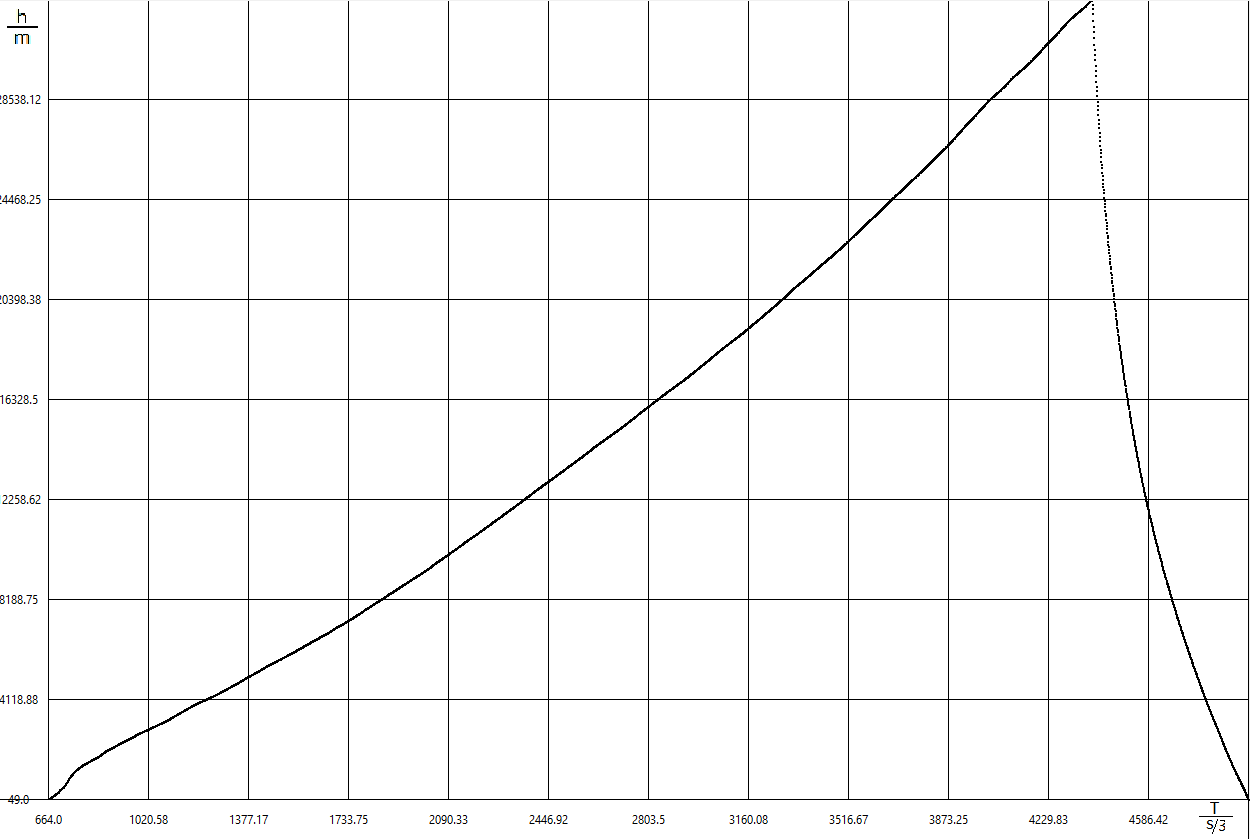
\includegraphics[width=1\textwidth]{NK_H_T.png}
	\caption{Kõrguse sõltuvus ajast}
	%\allikas{Minu programm}
	\label{NK_H_T}% Selle järgi viidatakse, see rida peab olema pärast \caption
\end{figure}


\subsection{Rõhu sõltuvus kõrgusest}
Joonisel \ref{NK_R_H} on näha rõhu sõltuvust kõrgusest. Graafikult tuleb ilusasti välja sõltuvus, välja arvatud umbes 10 km kõrgusel, kus jookseb kaks joont. Erinevus tekib, sest üks joon näitab andmeid tõusmisel ja teine langemisel.
\begin{figure}[h]
	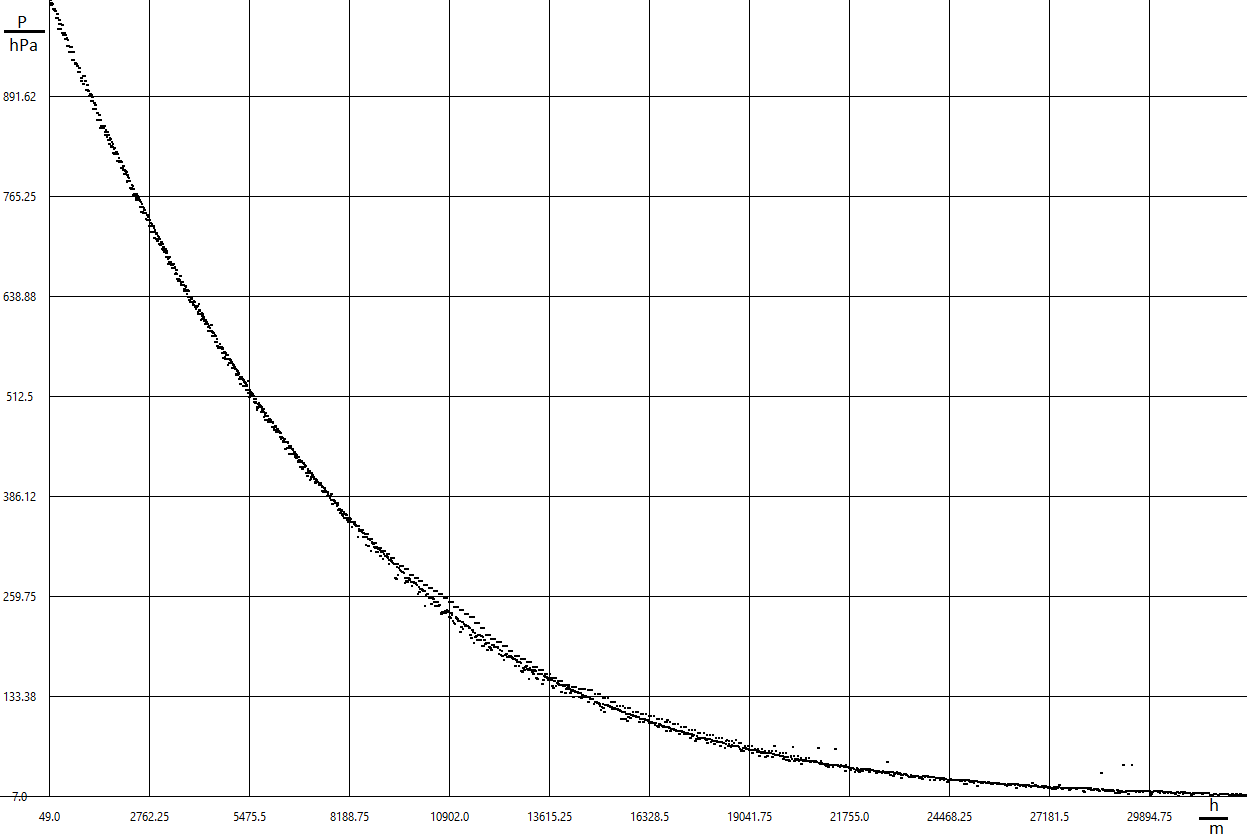
\includegraphics[width=1\textwidth]{NK_R_H.png}
	\caption{Rõhu sõltuvus kõrgusest}
	%\allikas{Minu programm}
	\label{NK_R_H}% Selle järgi viidatakse, see rida peab olema pärast \caption
\end{figure}

\subsection{Välistemperatuuri sõltuvus kõrgusest}
Joonisel \ref{NK_T_H} on näha välistemperatuuri sõltuvus kõrgusest. Nagu  joonisel \ref{NK_R_H} on ka siin näha kahte joont, mis tuleb tõusmisest ja langemisest. Tõusmisel on andmepunktid väga laiali valgunud, mis tuleb sondi pöörlemisest. Vahepeal on temperatuuri andur päikese poole, mille tõttu temperatuur on suurem ja vahepeal on andur päikesest eemal, mis juhul mõõdetakse tegelikku temperatuuri. Langemisel on pöörlemist vähem ja siis on punktid rohkem ühe joone peal. Et enda katses vältida andmete laialivalgumit, on vaja lahendada päikesest tulenevat temperatuur väärmõõtmise probleemi.
\newline On näha, et temperatuur ei lange pidevalt atmosfääris tõustes. Troposfääris temperatuur langeb, kuid strarosfääri jõudes hakkab temperatuur tõusma. Kõige külmem piirkond umbes 10 km kõrgusel.
\begin{figure}[h]
	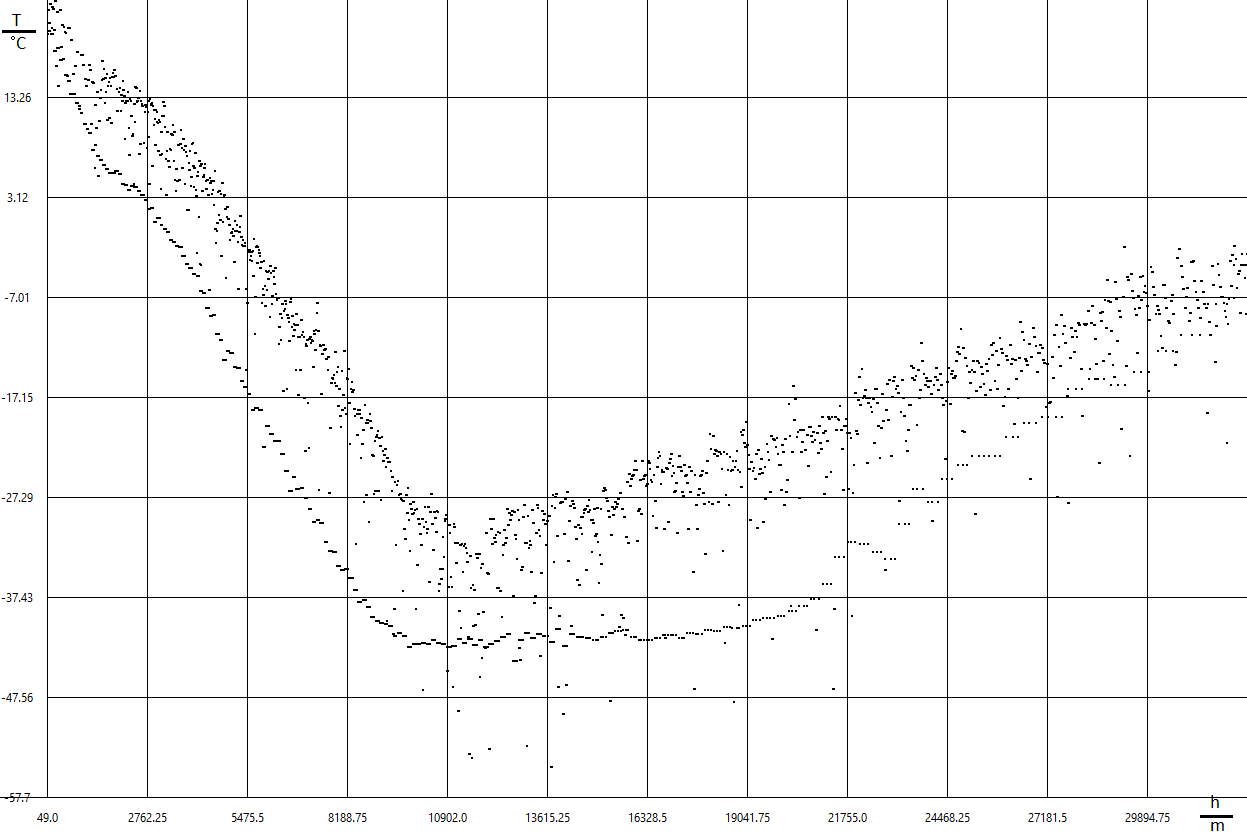
\includegraphics[width=1\textwidth]{NK_T_H.png}
	\caption{Välistemperatuuri sõltuvus kõrgusest}
	%\allikas{Minu programm}
	\label{NK_T_H}% Selle järgi viidatakse, see rida peab olema pärast \caption
\end{figure}


 
\addchap{Kasutatud materjalid}% Viitamine paraneb veel

Hobbs, P. V., Wallace, J. M. (2006) Atmospheric Science: An Introductory Survey. Amsterdam: Elsevier \newline
Ahrens, C. D., Henson, R. (2018) Meteorology Today: An Introduction to Weather, Climate, and the Environment. Boston: Cengage Learning

%\cite{examplebook}% Kõige lihtsam viitamise käsk 
%\cite{examplearticle}
%\cite{exampleonline}

%\printbibliography% Selle käsuga trükime kasutatud materjalid, kommenteeri see kiirema kompileerimise jaoks

%\appendix% Lisad
%\chapter{Kes see lisatööd ikka teha tahab}% Lisa pealkiri

\kinnitusleht% Kinnitusleht
\end{document}
